\documentclass[]{spieman}

\usepackage[utf8]{inputenc} \usepackage{amsmath,amsfonts,amssymb}
\usepackage{graphicx} \usepackage{grffile} \usepackage[colorlinks=true,
allcolors=blue]{hyperref} \usepackage{pdflscape} \usepackage{afterpage}

% Title definition
\title {The WIYN One Degree Imager in 2018: An Extended 30-Detector Focal Plane}

\author[a,b]{Daniel R. Harbeck} \author[c]{Mike Lesser} \author[b]{Wilson Liu}
\author[d]{Bob Stupak} \author[d]{Ron George} \author[d]{Ron Harris}
\author[d]{Gary Poczulp} \author[d]{Jayadev Rajagopal} \author[e]{Ralf Kotulla}
\author[c]{David Ouellete} \author[e]{Eric Hooper} \author[e]{Michael Smith}
\author[e]{Dustin Mason} \author[f]{Peter Onaka} \author[f]{Greg Chin}
\author[d]{Emily Hunting} \author[d]{Robert Christensen}

\affil[a]{Las Cumbres Observatory, Goleta, CA (USA)} \affil[b]{WIYN Observatory,
Tucson, AZ (USA)} \affil[c]{The University of Arizona, Tucson, AZ (USA)}
\affil[d]{NOAO, Tucson, AZ (USA)} \affil[e]{University of Wisconsin, Madison, WI
(USA)} \affil[f]{University of Hawaii, Honolulu, HI (USA)}

\newcommand{\electron}{e$^-$\xspace} \newcommand{\degree}{$^\circ$\xspace}


\begin{document}

\maketitle

\begin{abstract}
    
We report on the performance of the upgraded One Degree Imager (ODI) at the WIYN
3.5 meter telescope at the Kitt Peak Observatory. The focal plane has been
expanded by additional seventeen detectors in spring / summer 2015. The now 
thirty
Orthogonal Transfer Array CCD detectors provide a total field of view of 40’ x 
48’ on the
sky. The newly added detectors underwent a design revision to mitigate reduced
charge transfer efficiency under low light conditions (fat zero problem). We
discuss the performance of the focal plane and challenges in the photometric 
calibration of
the wide field of view, helped by the addition of telescope baffles. In a
parallel project, we upgraded the instrument's filter mechanism, where a
degrading worm-gear mechanism was replaced by a chain drive that is operating
faster and at a higher reliability level. Two more filters, a U band and narrow
band filter were added to the instrument's complement. We will review the
lessons learned during nearly three years of operating the instrument in the
observatory environment and discuss infrastructure upgrades that were driven by
ODI's needs. 

\end{abstract}


%>>>> Include a list of keywords after the abstract

\keywords{Ground based instrumentation, wide field imaging, CCD, Orthogonal
    Transfer Array, Observatory Operations}

%%%%%%%%%%%%%%%%%%%%%%%%%%%%%%%%%%%%%%%%%%%%%%%%%%%%%%%%%%%%%
\section{Introduction}

The One Degree Imager (ODI) has been the major instrument development project
from 2002 to 2015 at the WIYN 3.5 meter telescope (Kitt Peak, Arizona), and its design and 
progress has been documented in various SPIE conference contributions
\cite{jacoby2002, Harbeck2008, Jacoby2008, Yeatts2008, Harbeck2010, Yeatts2010, 
harbeck2014, gopu2014}. The instrument is designed for a one degree  square 
field of view with 64 Orthogonal Transfer Array (OTA) CCD sensor. A first 
incarnation of ODI was deployed in the summer of 2012 with a partially 
populated focal plane (with 13 out of 64 detectors installed); this  
incarnation of ODI was called pODI and was described in detail at the SPIE 
Astronomical Telescopes + Instrumentation conference in 2014\cite{harbeck2014}. 
In that paper we outlined an incremental upgrade path for the instrument to a 
larger focal plane; we have followed that path, In 2015, ODI was upgraded and 
deployed at WIYN  with an enlarged 5x6  detector array by adding 17 new detectors;
this incarnation of ODI is generally  referred to "5x6 ODI", or simply ODI, as no
additional development of the focal plane is planned at this point. In this paper we report 
on the status of the instrument after this upgrade. 


\section{Upgrade of the Instrument} 

ODI is designed to use Orthogonal Transfer Array (OTA) CCD detectors that have the unique
capability to move charge on both imaging dimensions during an integration in order to compensate for 
unwanted image motion. This concept has been demonstrated in pODI.  The detectors in pODI (production Lot 6)
had problems with (i) amplifier glow and (ii)  charge transfer efficiency under low light level conditions 
("fat zero" problem). The amplifier glow is mitigated by throttling the output drain voltage of the detectors 
during integration. The fat zero problem was traced to a structure between the imaging area and the serial output register. 

A  12 wafer demonstration run (Lot 7) showed that the low light level transfer inefficiency issue was 
resolved by a modification\cite{harbeck2014}, and all wafers of that batch were processed 
into packaged detectors at Imaging Technology 
Laboratory (ITL, Tucson, AZ),  yielding a total of 16 operational  Lot 7 OTA detectors that were 
designated for the ODI focal plane. After  processing these wafers, the 
processing equipment for ODI OTA detectors has been retired at ITL. 

The instrument was taken out of commission for upgrading from November 2014 to 
May 2015. The focal plane was immediately removed from the instrument and sent 
to  Imaging Technology Laboratory  (ITL) in Tucson, AZ to add the 16 new 
detectors; an additional Lot 6 device was identified and added to the focal 
plane as well. The 14 Lot 6 and 16 Lot 7 detectors were mounted on the focal 
plane to result in a contiguous 4x4 area of Lot 7 detectors, with the remaining 
Lot 6 detectors filling up an area to a 5 by 6 detector array (See Figure \ref{fig_focalplane}).


\begin{figure}
	\centering
	\hfill
	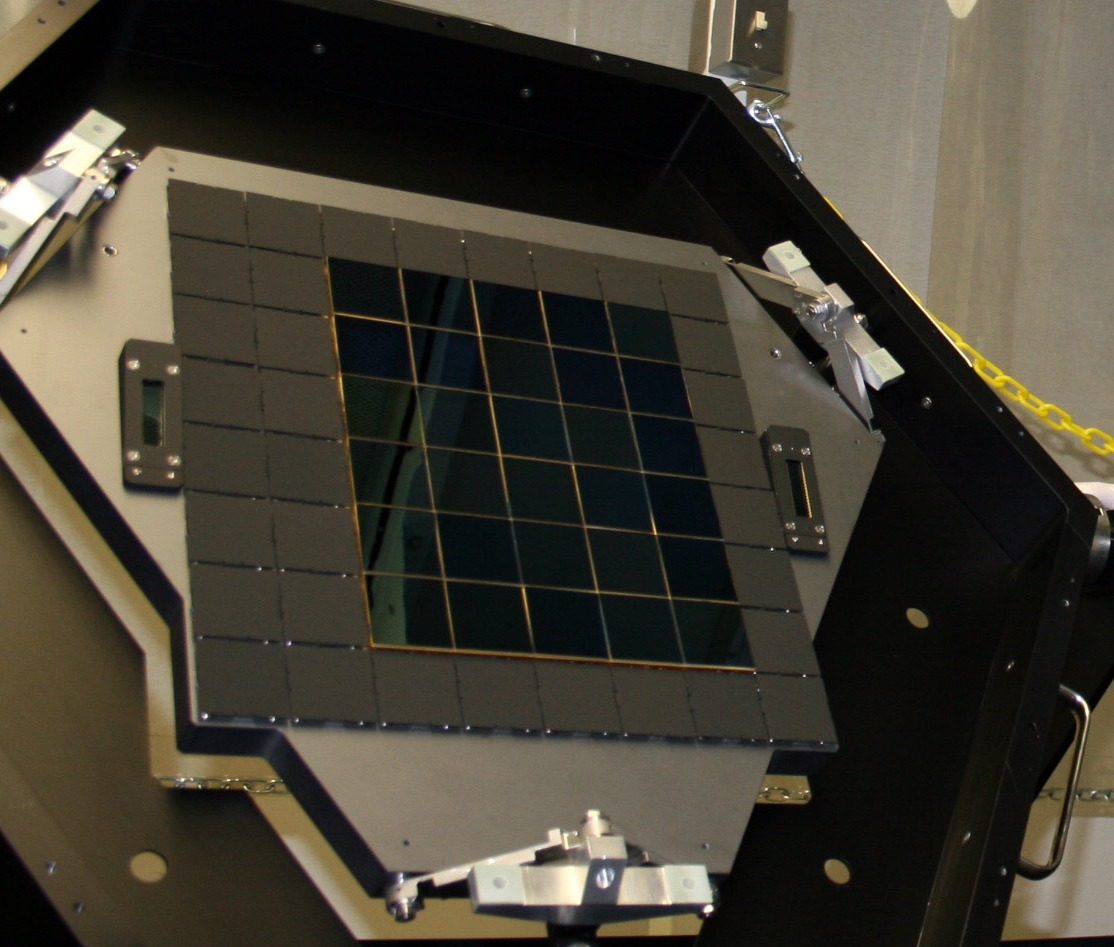
\includegraphics[height=0.4\textwidth]{images/detectorsOnFocalPlane5x6.jpg}
	\hfill
	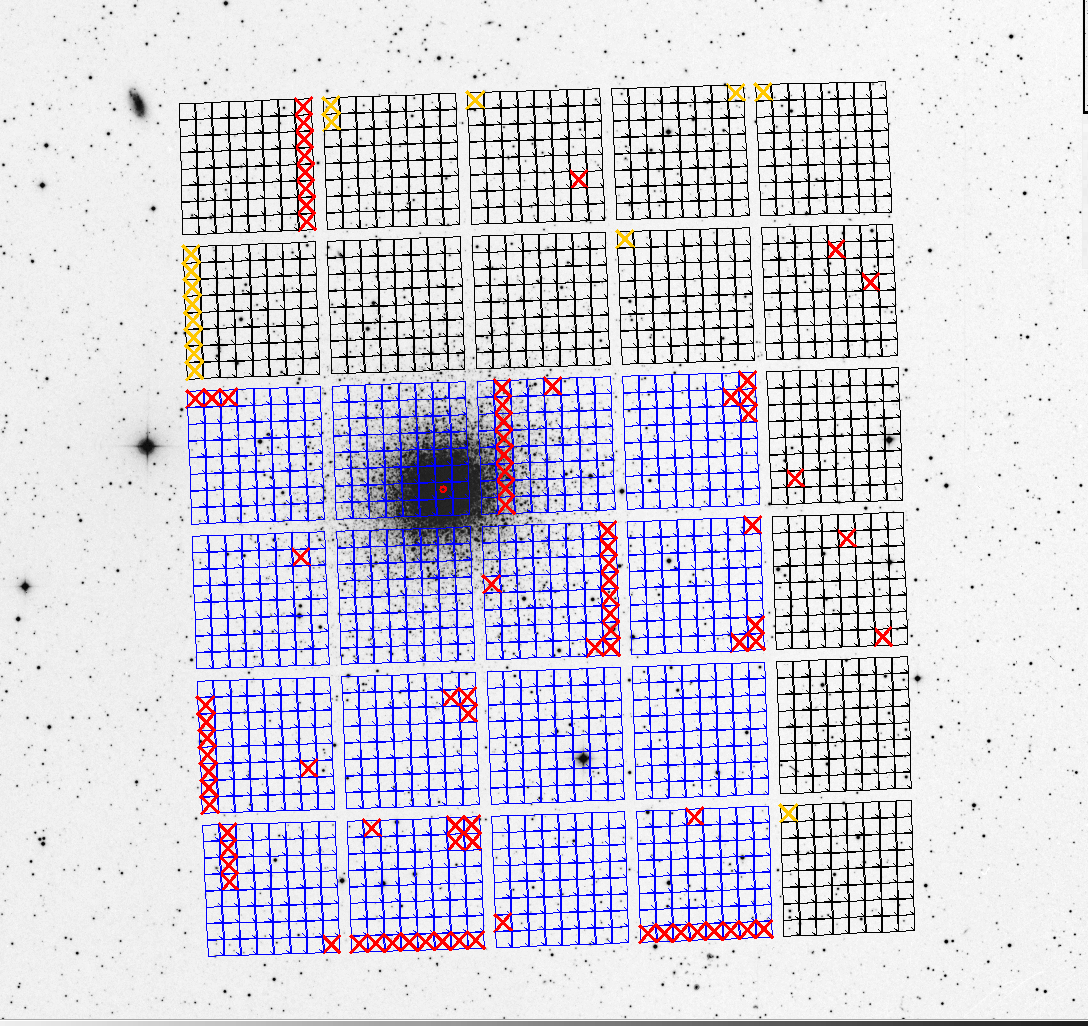
\includegraphics[height=0.4\textwidth]{images/5ODI_Imprint.png}
	\hfill \\[1ex]
	
	\caption{\label{fig_focalplane} Left: Upgraded focal plane with 30 
	detectors installed in a 5 x 6 array. The remaining detector positions are 
	covered with blackout plates to prevent stray light. Right: Imprint of the 
	detectors on sky. the total field of view is of order of $40'\times 48'$. 
	Known defective cells are marked with a red cross. }
\end{figure}


While the focal plane was repopulated with detectors, the cryostat and the 
instrument hardware were refurbished. We found in particular:
\begin{itemize}
	\item Some epoxy-sealed vacuum feed throughs had developed  leaks. We 
	attribute those to the thermally cycling casued by the nearby CCD controllers. 
	The daytime idle position of the instrument was changed to prevent the 
	formation of heat pockets near the vacuum seals, and to allow a better
	convective cooling flow in the CCD controller chassis.
	
	\item Inside the dewar we have identified areas of outgassing residue; 
	those areas have been cleaned. 
	
	\item The optical surfaces of ODI's corrector optics needed cleaning,
	 including the inside of the cryostat's dewar window. 
	
	\item The lubricant in a ring bearing for the atmospheric dispersion 
	corrector (ADC) prism had separated, and the liquid oil component started to 
	flow over one of the prisms. The optics were cleaned with no detrimental effect 
	to the surface and anti-reflection coating. Since the ADC bearings operate 
	only at a very slow speed, the lubricant had been entirely removed from the 
	ring bearings to avoid the risk of future leaks. 
	

\item  At the time of the dewar refurbishment, the molecular 
sieve material in the dewar (Zeolite 5-A) had lost its ability to adsorb gas in 
the dewar, leading to unmanageable short vacuum hold time of a few days only 
and it was hence  replaced with fresh material 5-A material. In the past, the 
Zeolite 5-A had been replaced on an annual basis due to its saturation. Since 
replacing the Zeolite in the dewar is an expensive and labour intensive operation, 
we started to investigate hydrophobic Zeolite ZSM-5 as a replacement candidate. Since 
ZSM-5 does not permanently bind water s 5-A does, it can be regenerated by vacuum 
pumping at room temperature. 

A year after the upgrade we found the Zeolite 5-A to  saturated again, and at that
time it was replaced with Zeolite ZSM-5. After more than three years of operations, 
the ZSM-5 material still performs well and shows no signs of saturation. We note 
that the ODI dewar is warmed up and vacuum-pumped a regular bases (every few months), 
which is regenerating the ZSM-5's ability to adsorb gas.
\end{itemize}

\subsection{Focal Plane  Performance}

as expected the Lot 7 OTA detectors performed similar to the Lot 6 detectors, but without the 
low light level charge transfer efficiency problem. Since the 5x6ODI focal plane  utilizes  both 
Lot 6 and Lot 7 detectors, observations that depend on the full field of view still
require minimum exposure level of the order of 100 electrons. If the smaller field of view of
the continuous Lot 7 sub-array is sufficient, those restrictions do not apply. The amplifier glow
observed in Lot 6 detectors remains unchanged, and is mitigated by throttling  the output drain 
voltage for all detectors but those that are used for guide star acquisition.

Controlling the output drain of the OTA detectors during integration and idling leads to a change 
in their power dissipation . We estimated the  difference between the
output drain on and off to about 0.5W per detector. Reading out the detectors with output drain on
will hence dissipate an additional 15 Watts into the focal plane for the readout time of about 6 seconds. 
This causes temperature variations in the focal plane of the order of several  few tens of to a full degree K, in
particular during a high cadence use cases. While the total cooling power of the
ODI focal plane would be sufficient to cool a focal plane that was populated with 64 OTA detectors, 
the temperature could not be held stable due to the need to throttle the output drain voltage during integration.


The Stargrasp CCD controller\cite{Onaka2008} used in ODI can control one or two detectors per board. For
pODI, a maximum of one detector was connected per CCD, and the cross-talk behaviour for two connected detectors was 
not yet demonstrated in ODI. In the 5x6 ODI focal plane, 2/3 of the detectors share a controller board, whereas 1/3
of the detectors are controlled by a single Stargrasp board each. No evidence of cross-talk between the two channels 
of a Stargrasp board was found. 



\subsection{Tuning the acquisition software}

The ODI data acquisition software is described in detail in previous SPIE
 contributions\cite{Yeatts2008,Yeatts2010}.
In short, the 5x6 ODI focal plane is read out by 20 Stargrasp CCD controllers which
interface to a network switch via individual  1GB ethernet over fiber
connections. The switch itself bundles the data connection into a 10GB network
backbone used by the ODI computers (three units with 24 cores, 32GB RAM each). The 
data stream from the 30 CCDS is collected by a single server / java virtual machine that is
managed by a JBOSS 5 application server. From there, data are saved to a storage device. 

The data rate has more than doubled (from 13 detectors to now 30) to about 1 Gigabyte that 
downloads from the detectors in about 6 seconds.  The scalability of
the data acquisition system was tested before the upgrade by creating a mock-up
focal plane  configuration to simulate the enlarged focal plane. This test
revealed some bottlenecks: the interval between sustained bias readouts
increased from about 25 seconds to over 40 seconds. Several bottlenecks in the
data acquisition code were identified and mitigated during the upgrade project
and commissioning phase:


\begin{enumerate} 
    
\item For pODI, all data were stored to NFS-mounted storage devices (Oracle ZFS appliance)
 and the delay in  write fits files to disk was the major factor to
slow down the data handling process. As a mitigation we equipped the acquisition
server with a Raid 5 configured local storage array, utilizing only disks with a
6G interface; new images are now first stored on the local hard drives. The image data 
are then slowly transferred by a background process to the storage appliance, 
both as a mid-term storage and to stage data for transfer into the ODI data archive.

\item   Simultaneously receiving of the data streams from 30 detectors via TCP/IP posed no
major challenge for the 10GB network backbone.  However, when writing the the
data to disk we realized a significant  improvement in the write speed by
limiting the number of data streams that are written in parallel to disk. As a
mitigation, the FITS file writing routine was changed into a Java {\tt Callable} that would
be submitted to a multi-threaded Executor, and we determined that ten storage threads delivered
a good performance. The write performance was further improved by rewriting the {\tt nom.tam.fits} package
to allow writing into {\tt BufferedOutputfile}. 

\item As part of the data storage process, a thumbnail image is generated for
each detector to help the observer to judge image quality in real time. For
pODI, the thumbnail generation was delegated to a command line utility that was
called after the images were written to disk, reading back (and decoding) the
fits file again. Also, the thumbnail generation process was unnecessarily
serialized in the data acquisition process, i.e., telescope observations would
be blocked until thumbnail images were generated.  For 5x6 ODI we have moved the
thumbnail generation into the Java virtual machine, were the data are already in memory, hence
saving I/O and CPU time for FITS decoding. Furthermore, the generation of the
thumbnails was delegated to  lower priority background threads, making the
thumbnail generation an asynchronous process.

    
\end{enumerate}

As indicated by prior testing, the existing IT infrastructure was capable of
handling the larger focal plane after some investments into faster local
storage and by serializing the data storage  processes.  After each readout, about 6 seconds
are spend to flush the detector to remove residual charge, and the readout
overhead is now limited by the detector and telescope performance.


\section{Filter change mechanism upgrade and performance}


\begin{figure}[]
	\centering
	\hfill
	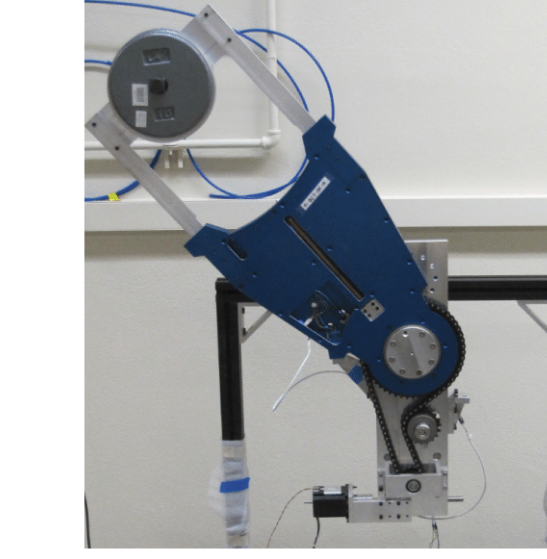
\includegraphics[height=0.49\textwidth]{images/filterdrivetest.png}
	\hfil
	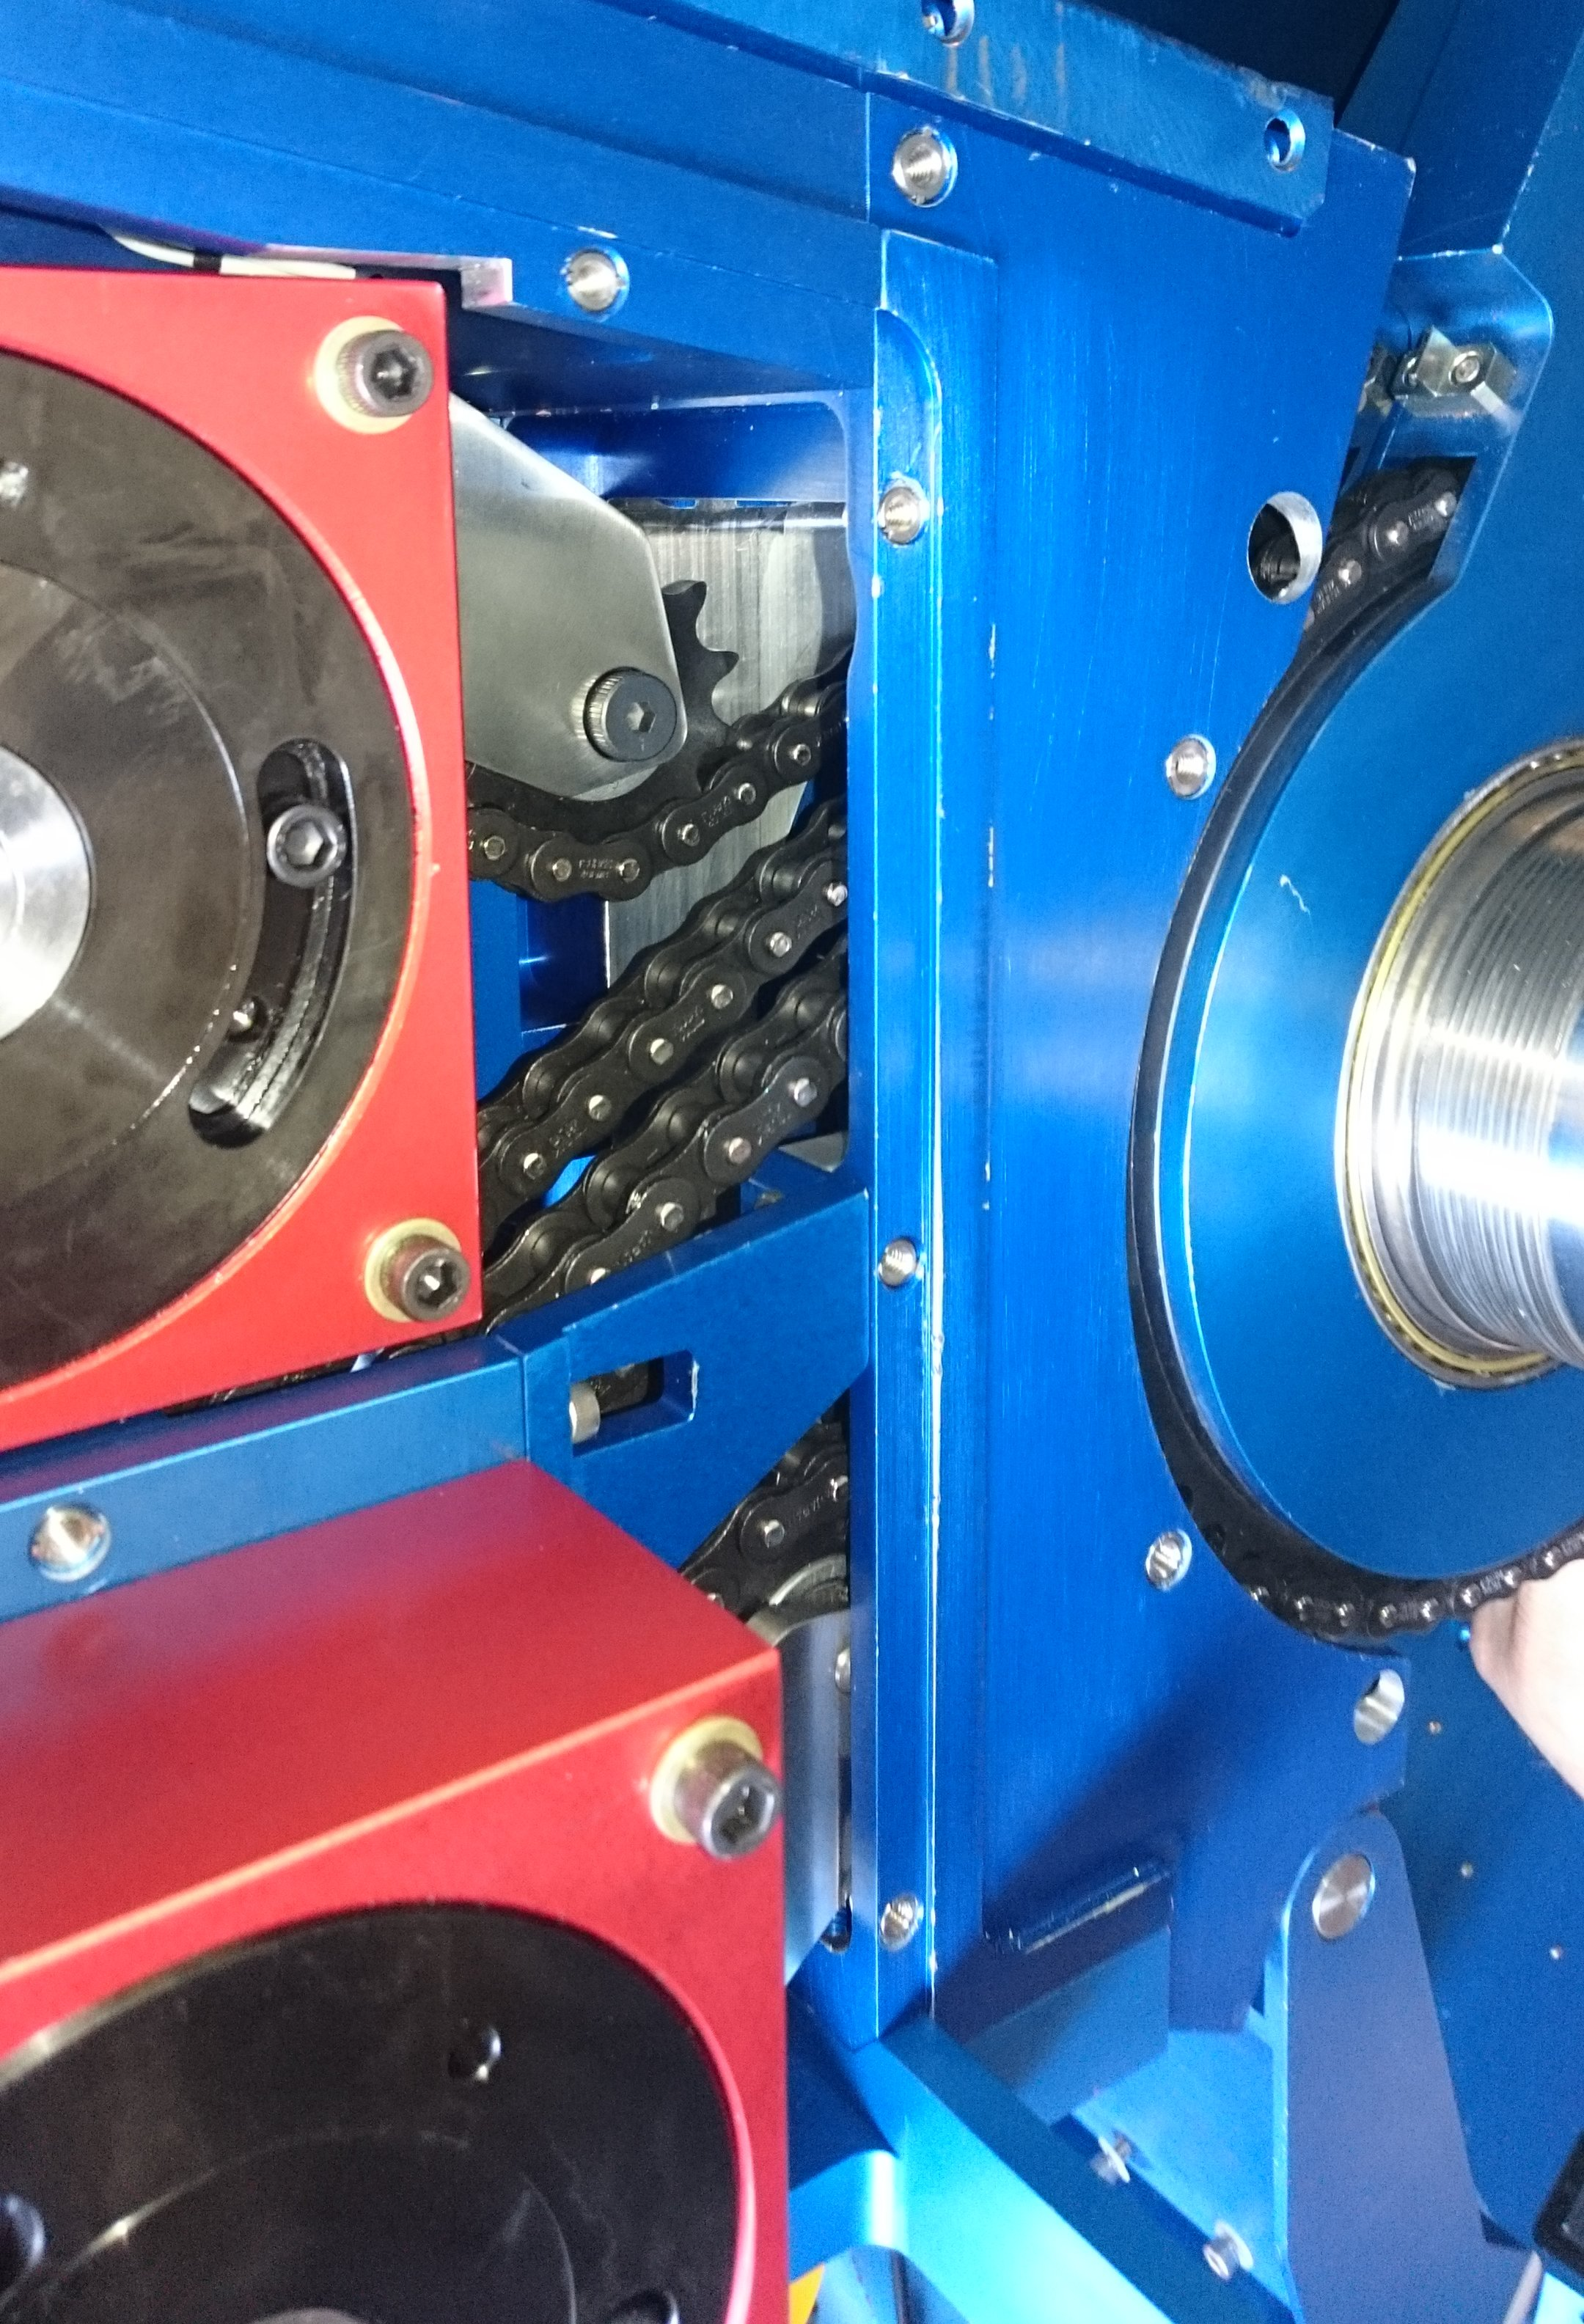
\includegraphics[height=0.49\textwidth]{images/DSC_0309.JPG}
	\hfill
	\caption{\label{fig_filterdrive} Left: Single filter arm test assembly. The 
		42x42 cm filter is simulated by a drive. This assembly was used to 
		stress-test the filter arm drive concept with order of six thousand in 
		and 
		out actuation. Right: Close-up of the three-filter layer assembly 
		during 
		installation at the instrument.   }
\end{figure}

ODI has a filter change mechanism that can hold up to nine filters, where each
filter is about 42cm by 42 cm in size. Each filter is inserted an removed out of
the beam by a semaphore-like filter arm that was originally driven by a worm
gear\cite{Muller2008}. Due to the proximity to optical surfaces, the worm gear
contact was operating without lubrication (steel on bronze contact). Already
during integration testing it was realized that this drive did not meet
requirements for operations, since as the stainless steel worm gear would slowly
shave of the bronze gear on the filter arm. However, due to time and resource
constraints this drive was deployed in operations in the pODI instrument, and
the bronze gear was replaced on an annual basis (and the instrument was then
cleanout out from bronze shavings, that at more than one occasion had caused
issues by shorting filter position switches.


In 2014 we have started a project to redesign the filter drive, where now 
instead of a worm gear the filter arm would be driven directly by a chain 
drive. The previously used custom-made gear box was replaced by a commercial, 
encapsulated lubricated worm gear. A single filter arm drive was build at UW 
Madison (Figure \ref{fig_filterdrive}, left), and the operation of the filter 
drive was successfully demonstrated for over 6000 actuation. After testing, the 
worm gear box was destructively opened and inspected for sings of wear - none 
was found. 
 
Upon successful testing, a full complement of nine filter drives were build at 
the NOAO instrument shop, and the upgraded filter drive was installed into the 
ODI instrument during the summer of 2015 (see Figure \ref{fig_filterdrive}, 
right). The new drive has worked without  errors ever after. 



\subsection{Straylight mitigation by additional baffles}

Before ODI was deployed, a detailed straylight analysis (Photon Engineering)
indicated that a significant contribution of off stray light can be expected to
fall onto the ODI focal plane. The two major contributors are (i) off-axis rays
reflecting off the tertiary mirror, then the primary mirror, and then entering
the instrument and (ii) off-axis rays reflecting off the tertiary mirror,
entering the instrument. The first stray light mode had already been addressed
by installing an additional baffle at the entrance aperture of ODI. The latter
stray light path, however, had not been mitigated yet. The impact of the
straylight is clearly visible in Figure\ref{fig_straylight}, where we show the
view through the instrument at the center and corner of the field of view.


\begin{figure}[]
	\centering
	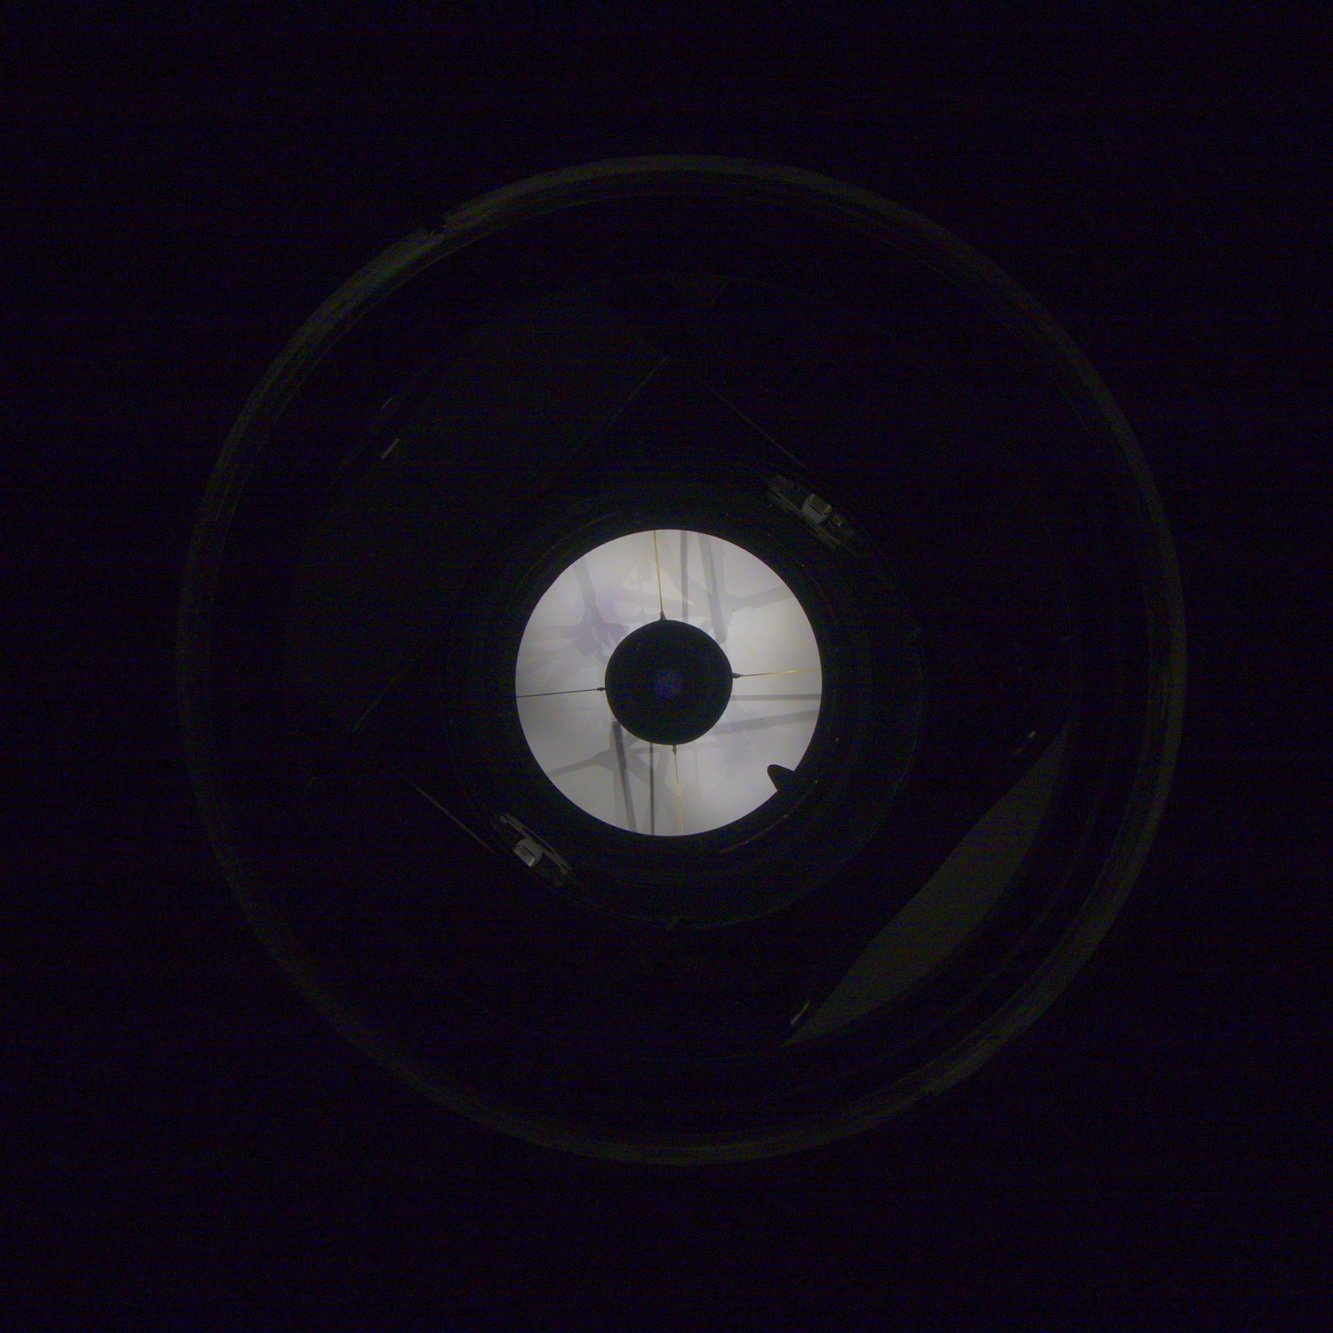
\includegraphics[width=0.49\columnwidth]{images/straylight-center.png}
	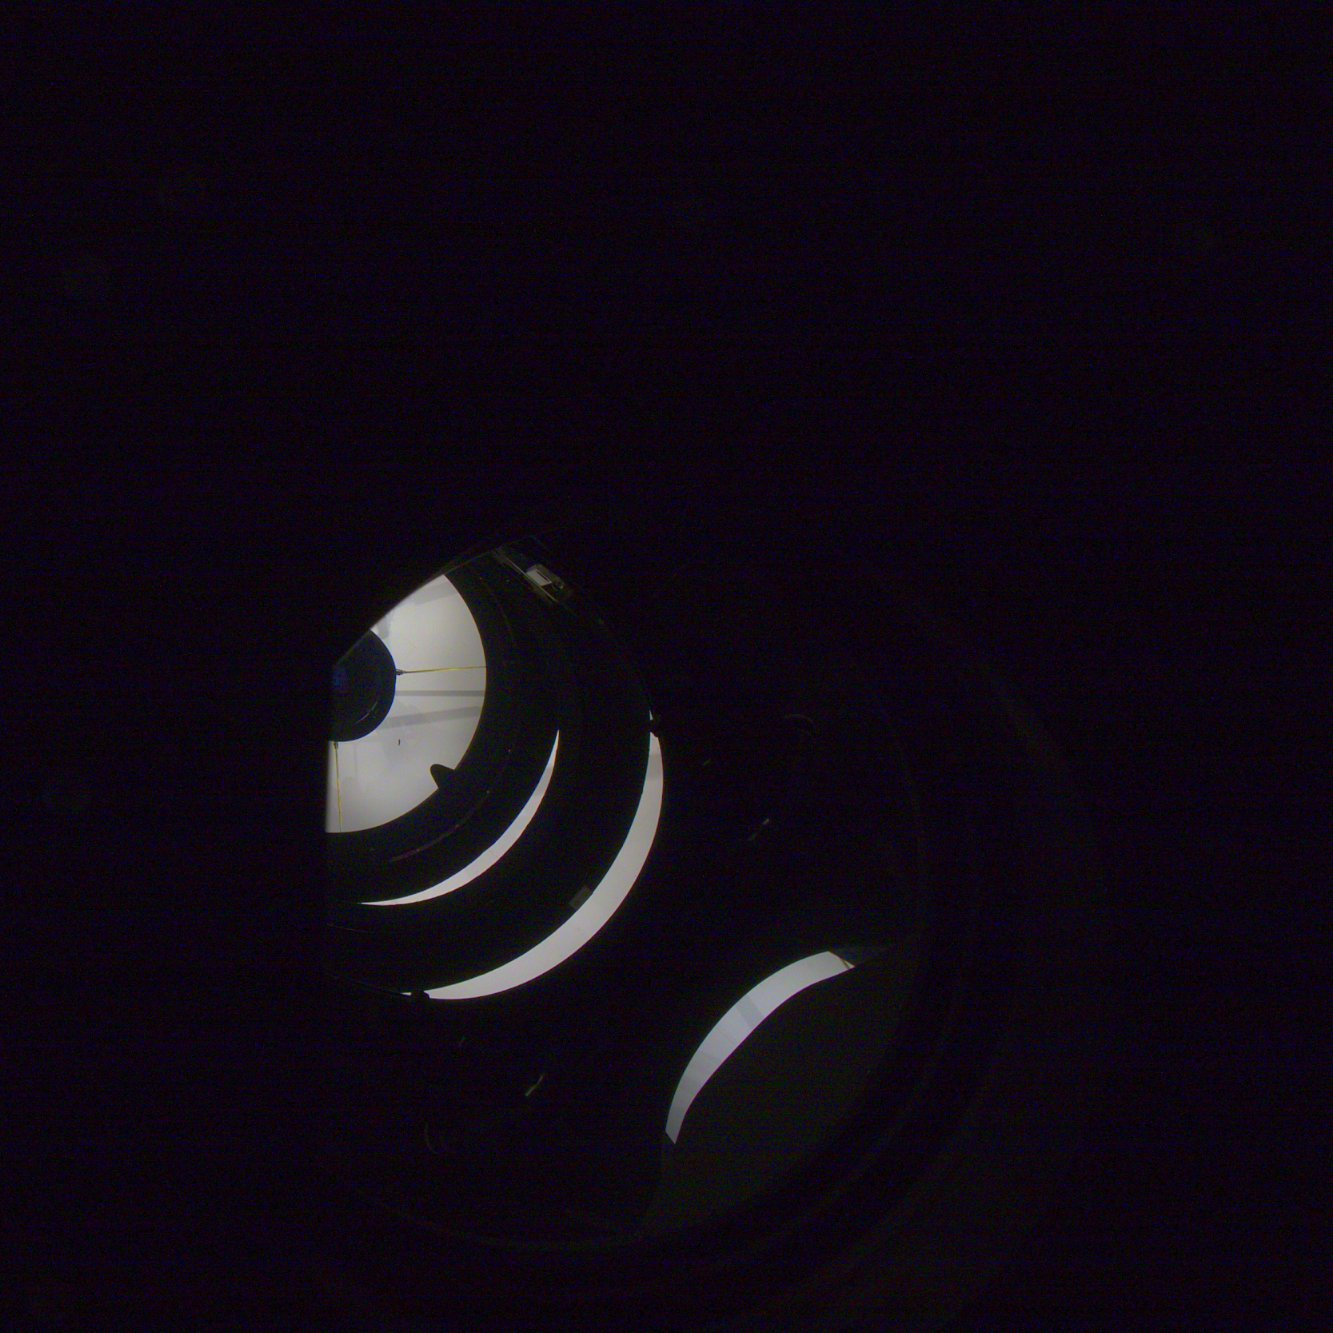
\includegraphics[width=0.49\columnwidth]{images/straylight-offcenter.png}
	\caption{\label{fig_straylight} View through the ODI instrument and 
	telescope
	onto the WIYN flat field screen. Left: at the center of the field, where 
	only
	the mirror pupil is a major contributor of illumination. Right: View from 
	the
	upper left corner of the instrument. Additional stray light arcs become
	visible. the upper two arcs originate from the off-field light that enters 
	the
	instrument directly off an reflection of the tertiary mirror. The third 
	lower
	right arc is due to reflection of off field light off the tertiary, onto the
	primary mirror, and  into the instrument. }
\end{figure}


While for the initial pODI instrument with a smaller focal plane the stray
light did not significantly affect operations, the extended focal plane of
ODI was found to be indeed heavily affected by the second stray light path.
For night time observations the straylight manifests in additional
background structure, it is detrimental for the acquisition of flat field,
where the stray light contamination was determined to be of order of 30\%.

The straylight is loopsided in the instrument, i.e., looking through the
Nasmyth port, only the upper left side of port would be affected by the
stray light. The instrument rotates at the Nasmyth port, and the effect of
straylight onto flatfields can be easily demonstrated by formatting the ratio
of two flat fields with the instrument rotated by $180^\circ$ with respect
to the telescope reference frame. Figure \label{fig_flatfieldbaffle}

\afterpage{%
    \clearpage% Flush earlier floats (otherwise order might not be correct)
    \thispagestyle{empty}% empty page style (?)
    \begin{landscape}% Landscape page
        \centering % Center table
        \begin{figure} \begin{tabular}{ccccc} odi u' & odi g' & odi r & odi
                i & odi z \\ \hline \multicolumn{5}{c}{ratio of $\pm 90 \deg$ flat
                    fields, no baffle} \\ \hline
                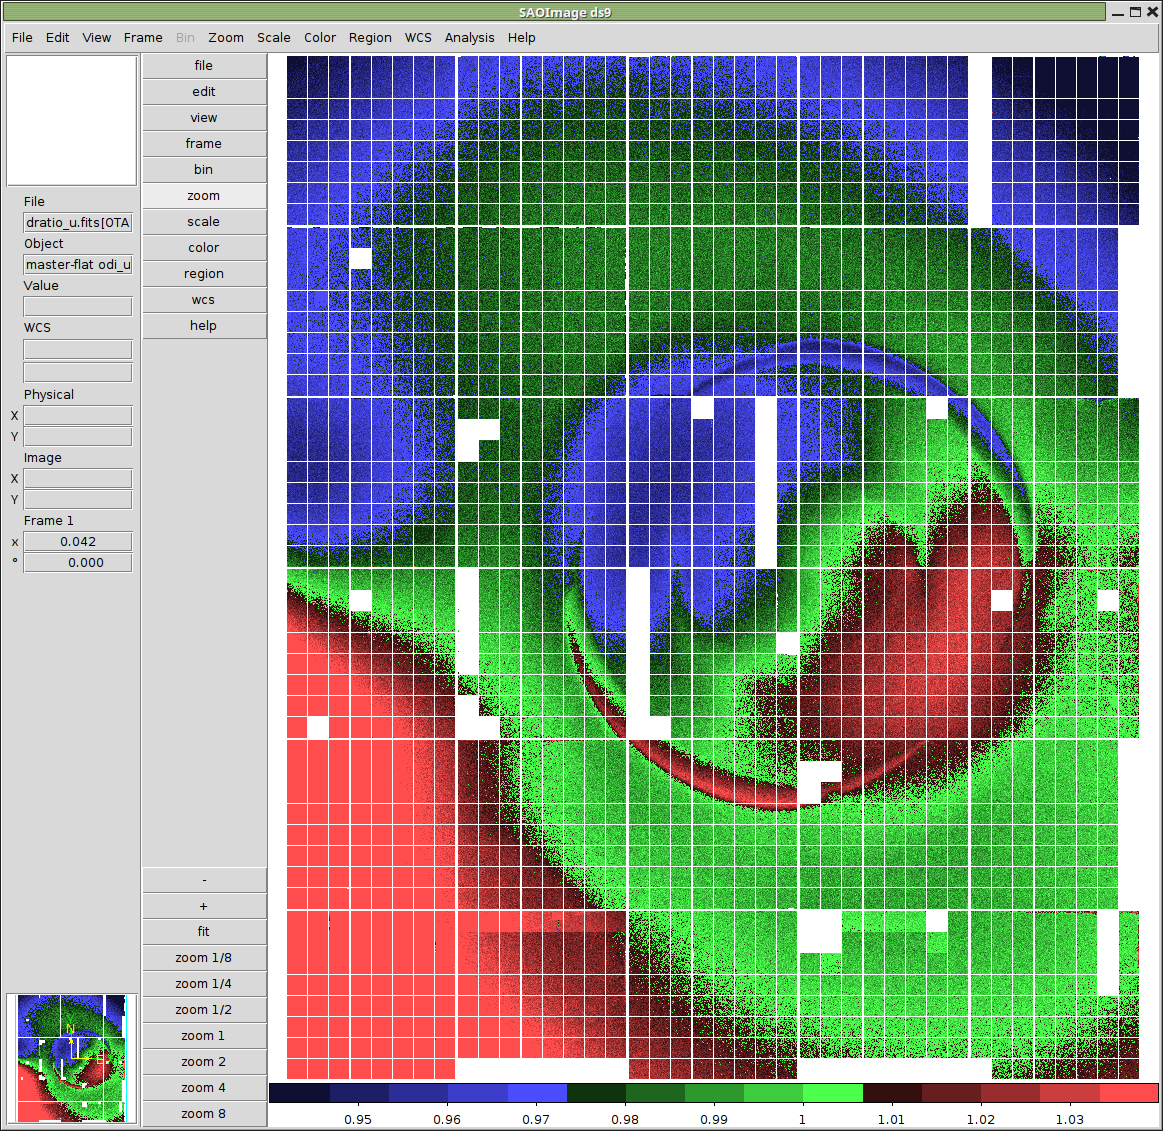
\includegraphics[width=0.2\textwidth]{images/nobaffle_u.png} &
                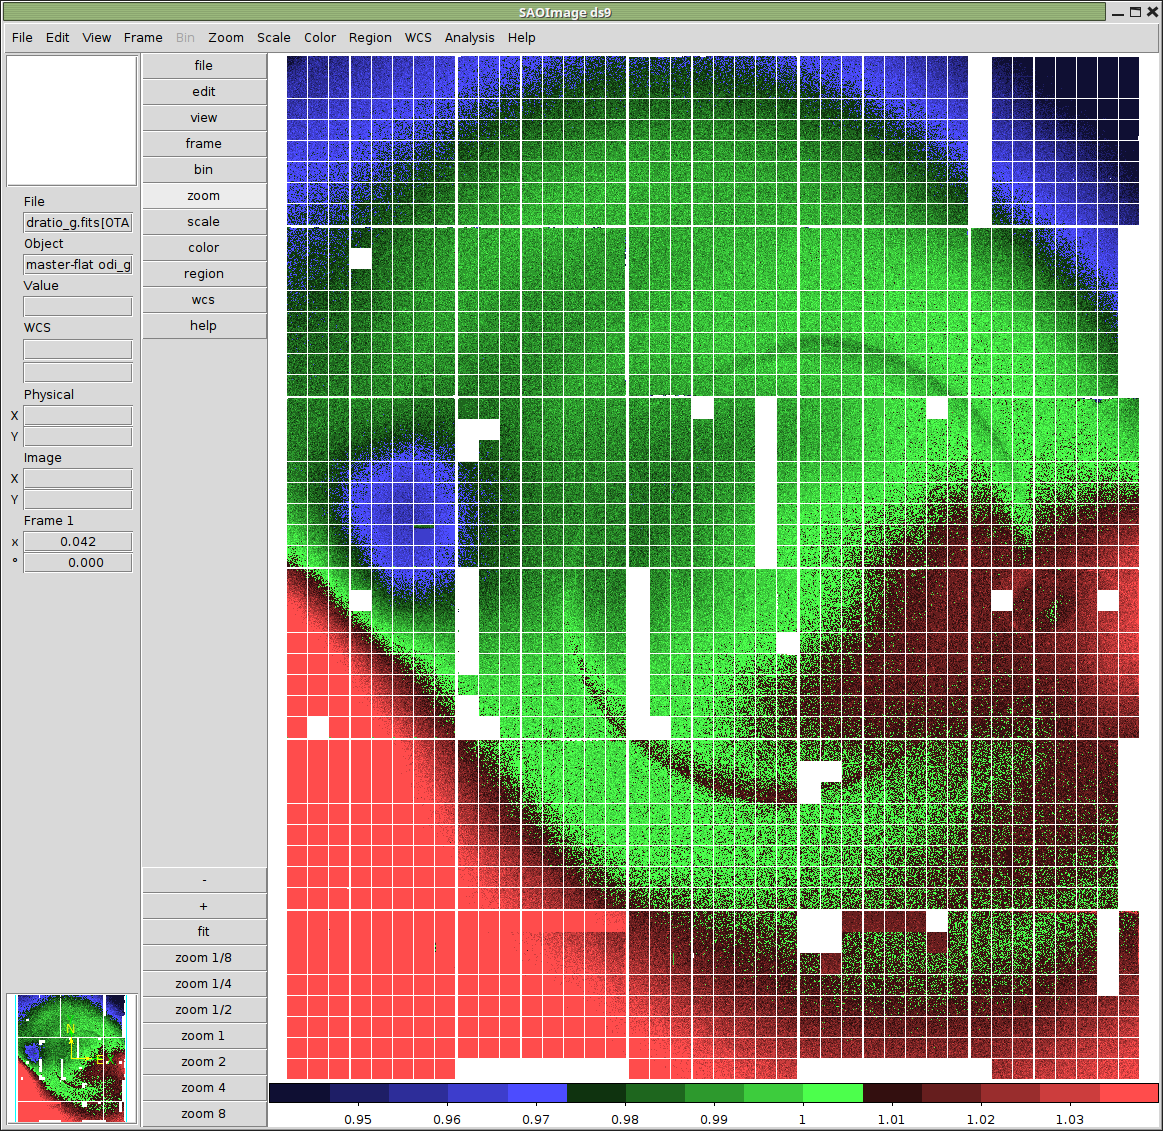
\includegraphics[width=0.2\textwidth]{images/nobaffle_g.png} &
                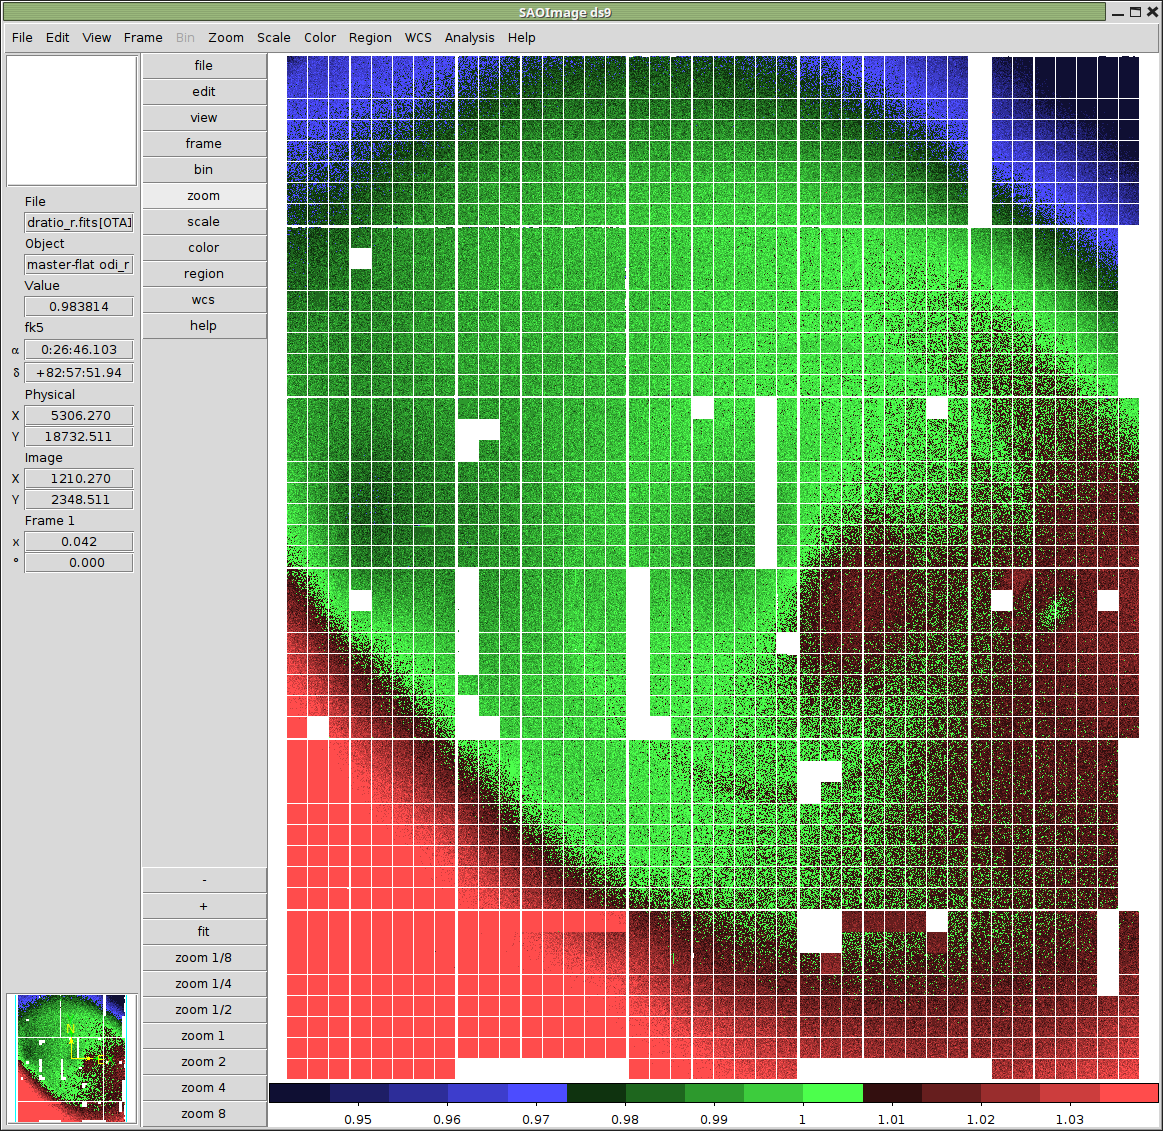
\includegraphics[width=0.2\textwidth]{images/nobaffle_r.png} &
                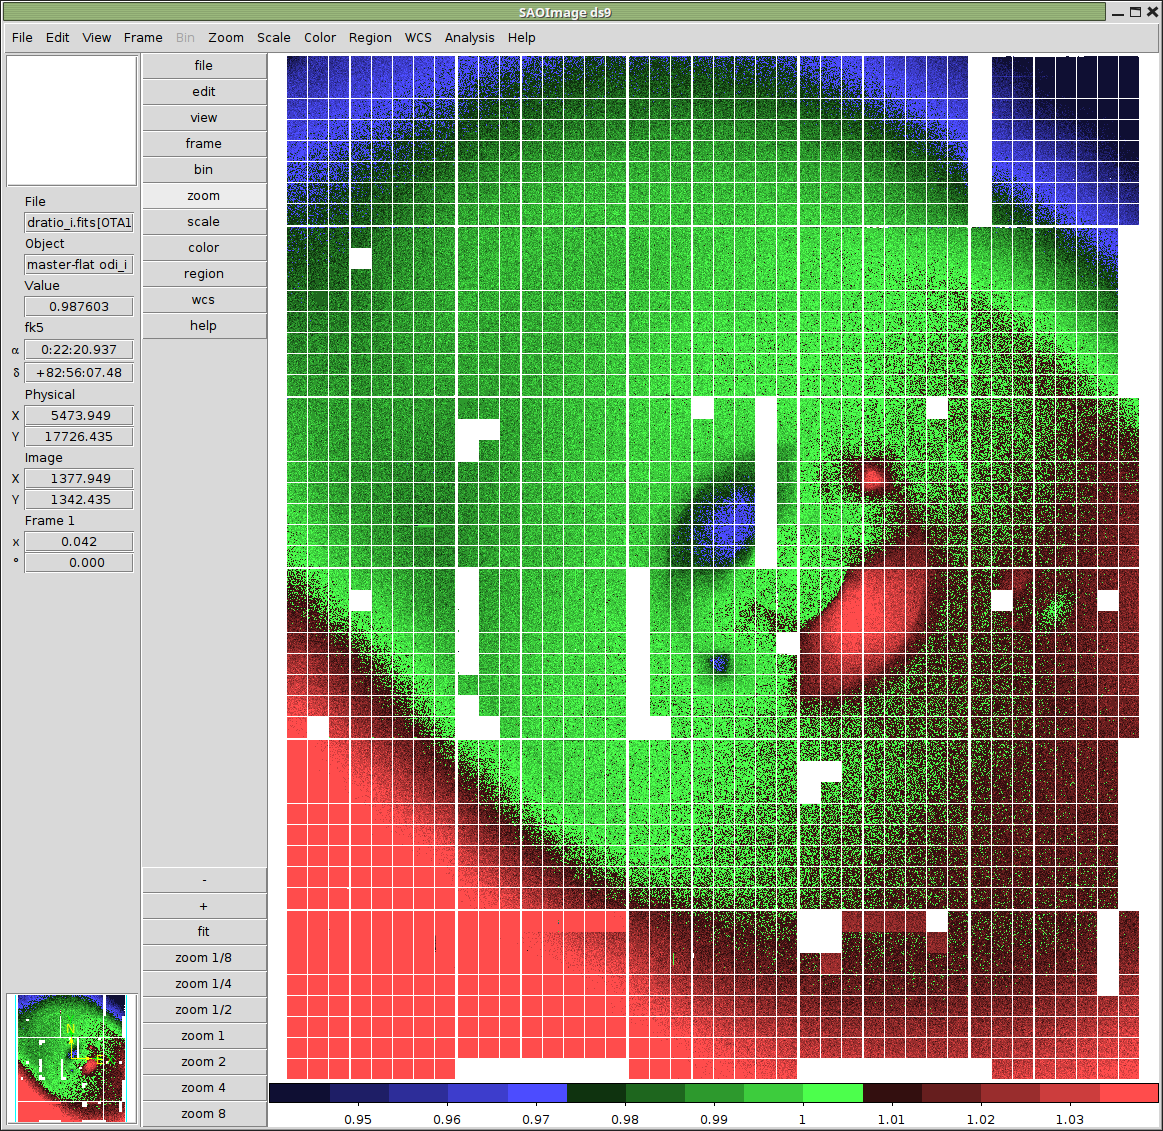
\includegraphics[width=0.2\textwidth]{images/nobaffle_i.png} &
                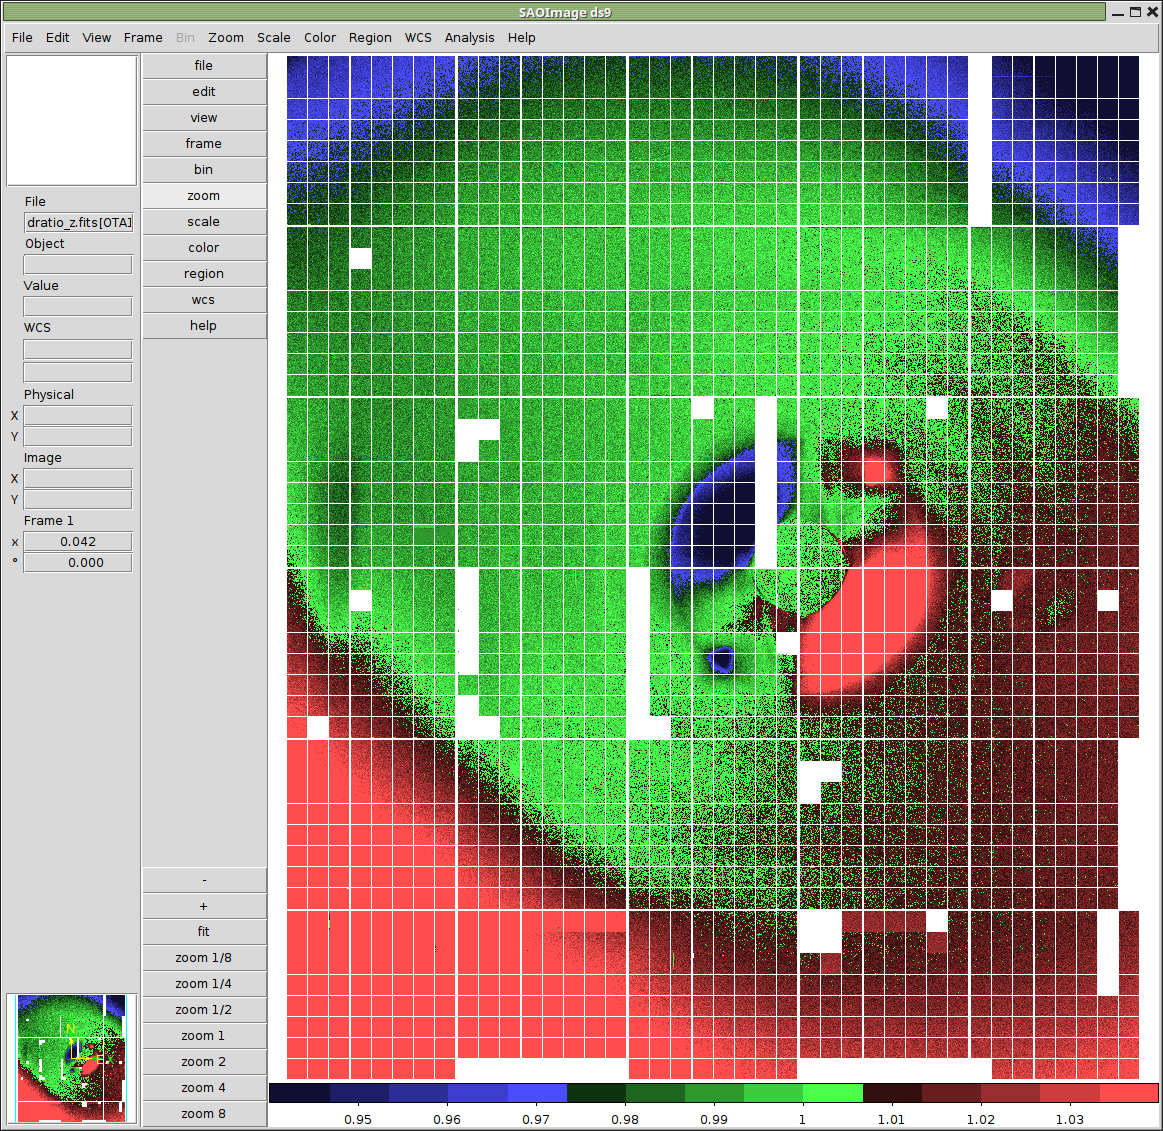
\includegraphics[width=0.2\textwidth]{images/nobaffle_z.png} \\
                \hline
                
            \end{tabular}
            
            \caption{\label{fig_flatfieldbaffle} Ratios of flat field images
                taken at an instrument rotator angle of $+90^\circ$ $-90^\circ$ 
                for all ODI broad band filters. }
            
        \end{figure}
        
    \end{landscape} 
  \clearpage% Flush page
}



\subsection{Pupil ghost suppression using a two bladed shutter}

Reflections of the optical surfaces within WIYN One Degree Imager (ODI) produce
internal ghosting, resulting inflat fields or exposures of the night sky to form
an image of the telescope pupil. Thanks to anti-reflection coatings on the
optics, each reflection is suppressed to about about 1\%-2\% level, depending on
the actual wavelength of the light, but the residual light is still capable of
producing a significant ghosting component. ODI’s dewar window is concave, and
paired with the plane surface of the passband filter forms an imaging system
that.

\begin{figure}
	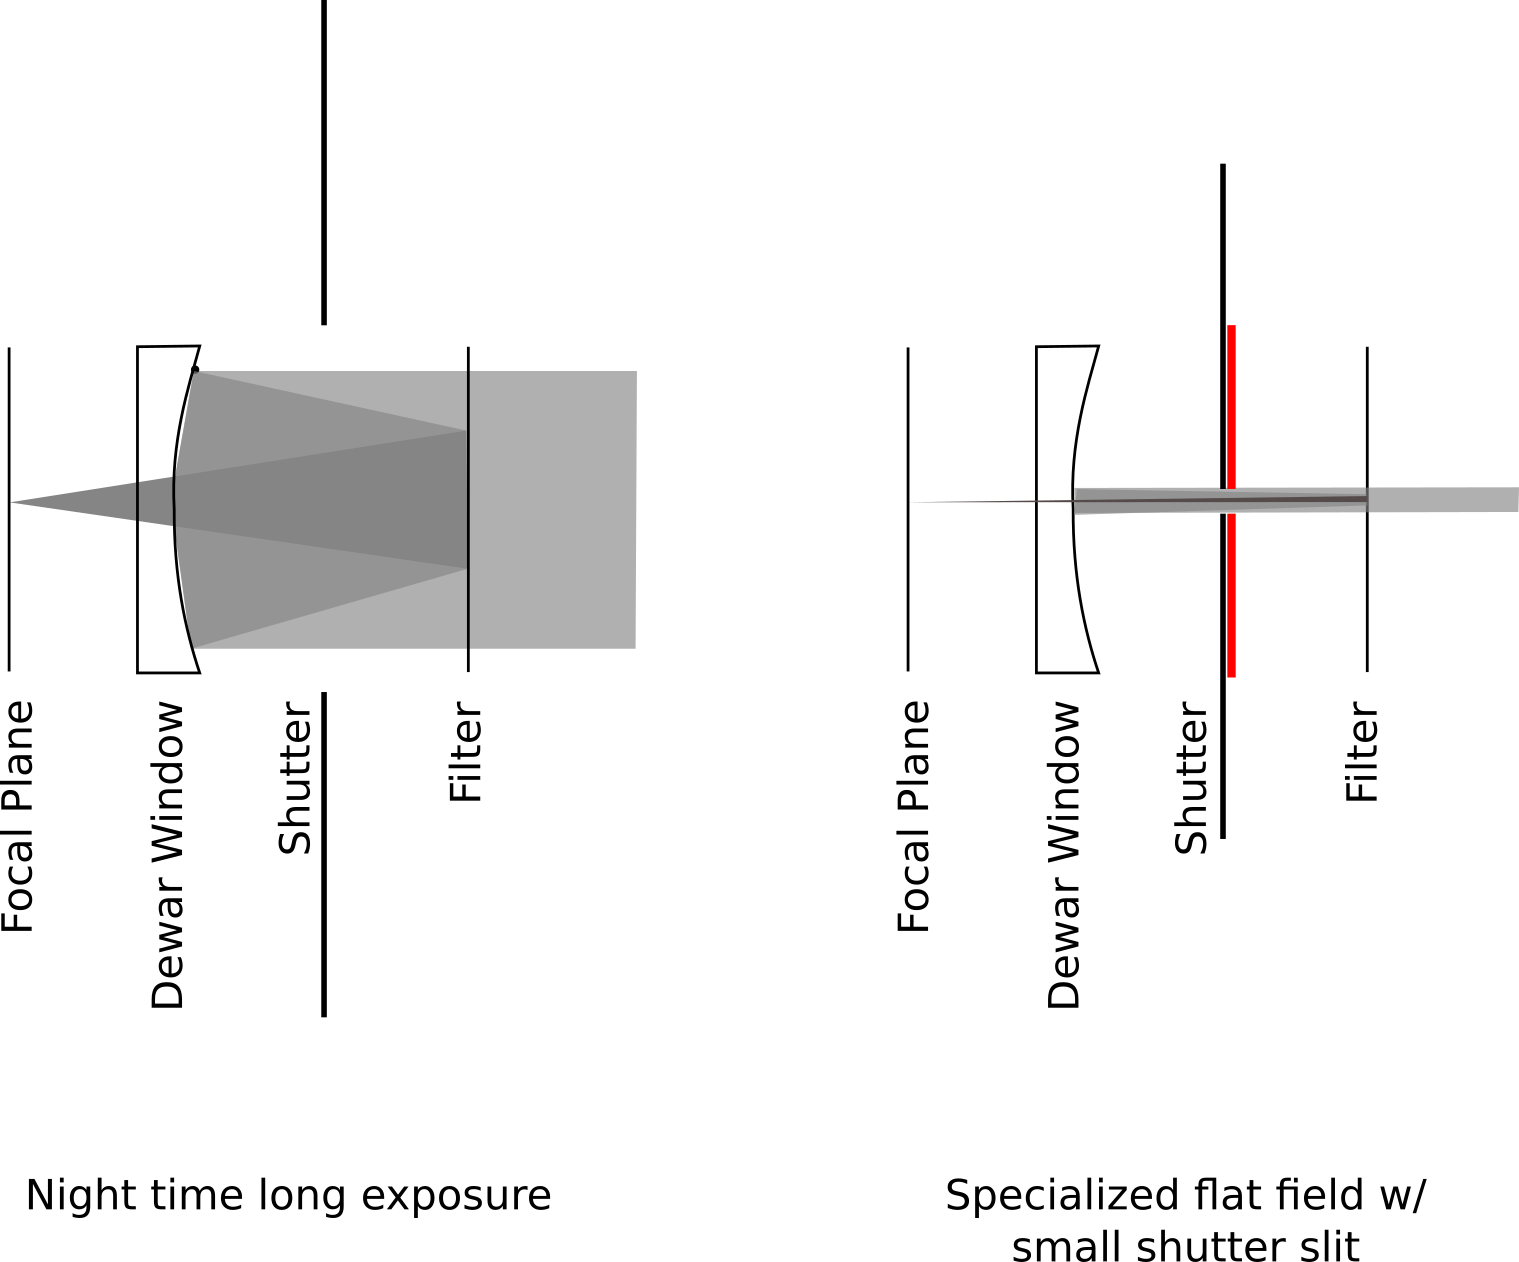
\includegraphics[height=8cm]{images/odishutterpupilghostsupression.png}
	\hspace{0.5cm} 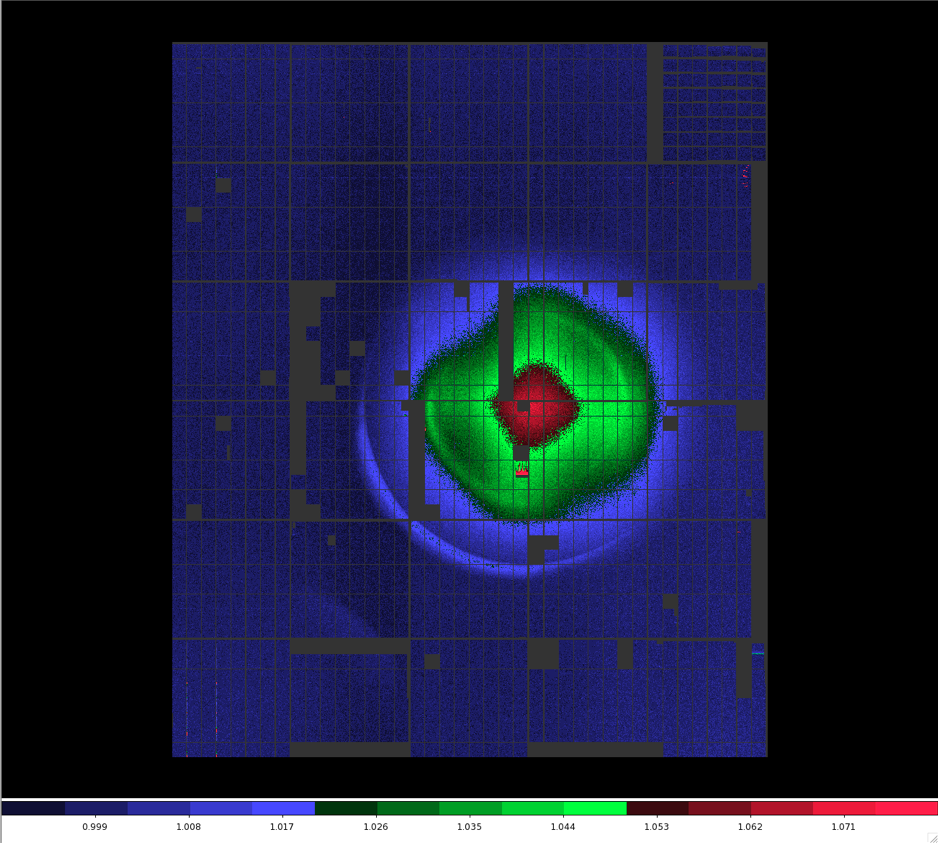
\includegraphics[height=8cm]{images/odi_layeronepg.png}
	
	\caption{ \label{fig_pupilghost}Left: Formation of the pupil ghost in ODI:  light 
		entering the instrument from the telescope (from the right) reflects of the
		concave dewar window, and the converging beam reflects of the filter to
		form an in-focus image of the telescope pupil. Right: Ratio of a flat
		field taken with different shutter modes. The sensitivity variations between
		pixels and detectors cancel out, but the excess ghosting light remains. Note
		that this ratio shows the ghosting component created by filters that are at
		a different location than in Fig. 1, and the pupil ghost is largely out of
		focus.}
\end{figure}

The excess light of the pupil ghost is undesirable for several reasons: In
night-sky observations it will produce an extra background component, but that
can be subtracted out. More severely, the pupil ghost also produces an extra
light component in a calibrating flat field, and if not treated, would lead to a
wrong sensitivity calibration in the affected areas.

The first method to remove the pupil ghost out of calibration images was to
model the ghost image and to then subtract it out of the flat field images. This
approach was overall successful, but is prone to adding noise and residual
errors from fitting a template to data. It remains desirable to avoid the pupil
ghost formation.

The pupil ghost was found to be greatly suppressed by the ODI shutter when the
exposure is tuned in a way where the shutter blades mostly obstruct the optical
path in front of the dewar window, and expose only via a narrow slit that moves
slowly over the focal plane. This suppression mechanism is illustrated by Figure
\ref{fig_pupilghost}. Note that, despite the shutter forming only a narrow slit,
the direct illumination of the focal plane is identical to a flat field where
the shutter completely opens.

This ghost-suppressing behavior of the shutter has been exploited already by
using very short exposure times of order of 50ms for sky flat fields, and this
new method has replaced the pupil ghost model subtraction method. However,
 this method was applicable only for situations with a very
bright flat field illumination that would support extremely short exposure
times. By lowering the travel speed of the shutter blades, however, one can
achieve the same ghost suppressing property at longer exposure times on the
focal plate. The cost, however, is that each flat field will take about 27
seconds longer, as this is the travel time of the blades (the travel time at
default speed is about 0.75 seconds).

A good demonstration of the pupil ghost suppression by the shutter is to divide
a flat field where the shutter is operated conventionally by a flat field where
the shutter was operated in the narrow-slit mode. Only the extra stray light
component should remain visible in the image, as demonstrated in Figure
\ref{fig_pupilghost}.


\section{Condensation}

A major operational limitation of ODI is the susceptibility of the dewar window
to condensation. As the condensation itself will evaporate quickly under dryer
conditions, we have found that inevitably a significant residue film would be
left that can only be removed by mechanical cleaning (drag wiping with alcohol).
The effect of the residue fil is detrimental for any scientific use of ODI,
since it causes significant scattering and halos around objects. Of the order of
50\%  of the light would be typically scattered from the PSF core into a bright
halo.

While the dewar window is surrounded by dry air outlets, we have identified
several scenarios in which the humidity near the window is insufficiently
controlled:

\begin{enumerate}
	\item {\bf The ambient humidity is above 70\% to 80\%}. The ODI instrument 
	was not designed as an airtight, or slightly over pressurized instrument, 
	and humid, ambient air can mix into the instrument cavity (the space 
	between dewar window and front lens, where the filter arms, shutter, and 
	atmospheric dispersion commentator are located).
	
	The initial design od ODI in fact foresees air to be actively removed from 
	the instrument cavity in order to force a slow flow of ambient air through 
	the instrument to improve thermal equalization. 
	
	Condensation typically appears when the shutter (located directly in front 
	of the dewar window) is opened. While the shutter is closed, the injected 
	dry air is confined to the small space between the dewar window and 
	shutter. Once the shutter is opened, the  humid air of the instrument 
	cavity mixes in, and condensation can form on the cold dewar window. 
	
	As immediate mitigation against condensation, operations of ODI are limited 
	to ambient humidity below 70\%RH.
	
	\item {\bf Failure in dry air supply:} The dry air for ODI is generated by 
	a dehumidifier. At several instances the supply has failed: Most often due 
	to a failure in the supplying air compressor (contactor failure or power 
	outages), but also due to a failure in the dehumidifier, or due to a 
	rupture in the dry air supply line. In order to protect against failures in 
	th edry air supply, we a redundant air compressor and a larger dry air 
	resoirvoir tank were installed at the telescope site. 

\end{enumerate}

Long term, a dewar window heater has to be installed  around the dewar window 
to prevent condensation. Such a heater would have to provide of the order of 60 
W power. Heater strips that can be glued to the perimeter of the dewar window 
are readily available, and a the dewar window mount allows for the addition of 
heaters with a modest machining effort.  


\section{Summary}

With the upgrade of the focal plane and the filter drives in 2015, the ODI
instrument has reached a stable state and is a scientifically useful instrument
for the WIYN community. With the upgrade of the filter arm mechanism, the
instrument infrastructure is robust, and only condensation of the dewar window
remains a limitation during  operations; condensation can be mitigated by the 
installation of heater on the circumference of the dewar window.

It has been demonstrated  that the tip tilt image motion can be
successfully compensated by OTA detectors, which was the original motivation to 
utilize OTA detectors in ODI.  However, the amplifier glow in ODI's OTAs 
prohibits the use of a detector for simulataneous guide star acquisition and 
sciene integration; localized atmospheric image motion compensation within an 
isokinetic patch is not achievable with the devices developed for ODI. Even 
if the amplifier glow were to be addressed
successfully, there are practical issues with implementing a rubber focal plane
as envisioned in \cite{tonry2002}: The density of  bright guide stars is
insufficient in some  optical passbands, in particular outside the galactic
plane. It is not sufficiently established how one would proceed to
astrometrically calibrate such a rubber focal plane.  Hence, neither the 
PanSTARRS survey nor the ODI instrument have operated the focal plane in the 
rubber mode beyond demonstration purposes.  I

ODI is now a mature instrument in routine operation. The choice to use  OTA 
detectors in ODI has significantly complicated the design, construction, and 
operation of the focal plane, including subsequent data calibration. However, 
no benefits from OTA detectors are derived for the ODI instrument. A change to 
conventional CCD detectors would be the next logical step in the evolution of 
ODI.
 
%%%% References %%%%%
\bibliography{odi} 
\bibliographystyle{spiejour}

\end{document}
